\section{Was there any conflict at River Corner Church growing up? How did your family relate to it? How was conflict resolved in your family in general?}
During my growing up years it seemed to me that most of the conflict at River Corner Church involved whether you had a first a radio and then a television.
I do not have memories of preachers preaching specifically about radios or televisions but rather that the way we live should remain separate from the world.
"Be not conformed to this world but be ye transformed by the renewing of your mind.
" Think of what is good and acceptable to God.
\begin{figure}
\centering
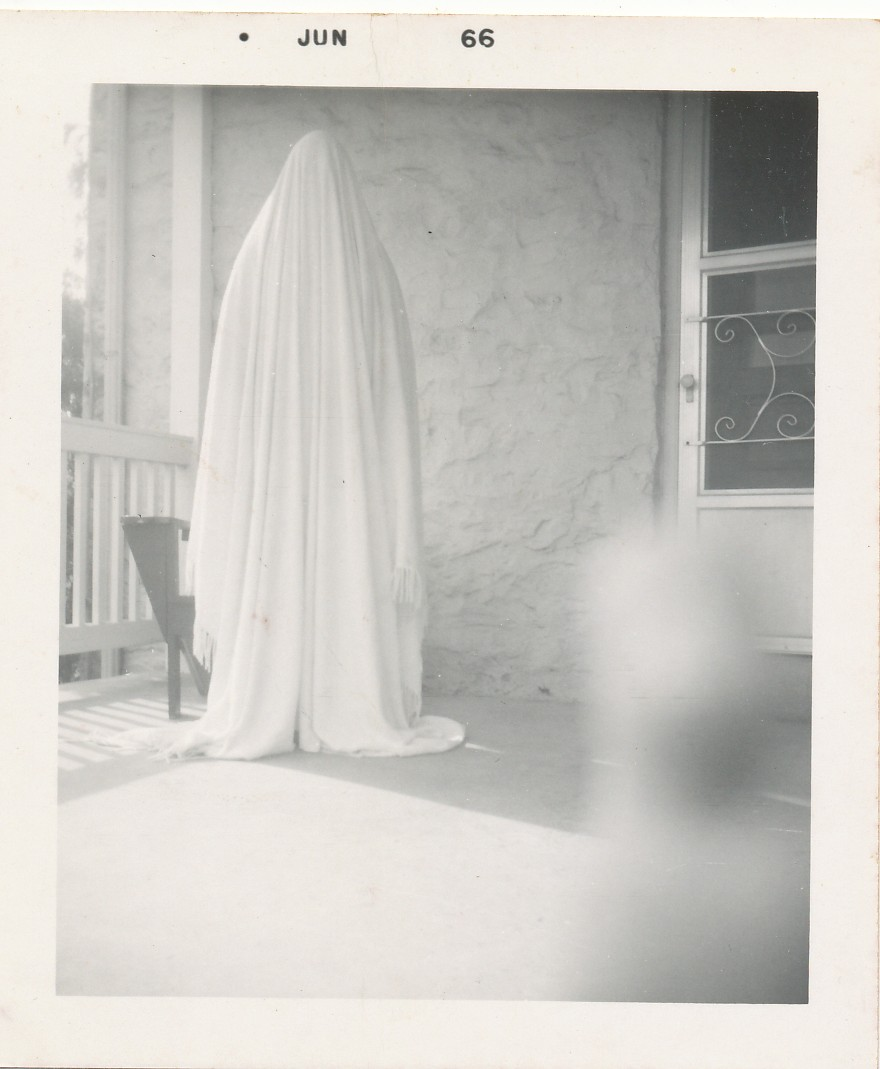
\includegraphics[width=0.9\textwidth]{finding_my_way/1.jpg}
\caption{
River Corner Mennonite Church
}
\end{figure}

There were concerns about the way one dressed as well.
If male, did you wear a plain coat or a lapel coat with a long tie? For women the concern was, the length of your dress, did you wear a cape as part of your dress and what was the size of your covering?
There was one man, Amos Shenk, brother of the preacher, who wore a bow tie under his plain coat.
Perhaps that was his small form of protest.

I do not know if the preacher confronted people who were out of line directly.
I think that he did not.
At least not very often.
The bishop for our church district was tolerant and seemed to choose not to make this a divisive issue and may have saved the district from splitting.
There were people in our congregation who left RC and went to the local Brethren in Christ Church.

My parents did not want my brothers to wear lapel coats and ties.
When they had their own money they bought what they wanted to wear.
My mother sewed dresses for her daughters so there was the tension of how we wanted the dress to look and how she was willing to sew the dress.
When Lancaster Conference Bishop Board changed their expectations for dress my parents said they no longer hold us to the earlier expectations.

I have to think about conflict in my family.
There was conflict from time to time.
Particularly as the family grew.
At times there seemed to be unspoken conflict between my parents.
I do not remember them openly arguing.
I remember that my father's style was to hold in what he was feeling and then there were a few times that in frustration he hit a teenager child.
I do not remember getting spanked but there were other siblings who did.
There was quite a bit of conflict between one brother and sister in their growing up years.
That got resolved along the way.
Perhaps my most common mode of operation was to observe what was happening among others in conflict without getting involved myself.





